

\documentclass[DIV=calc, paper=a4, fontsize=11pt]{scrartcl}
\usepackage{makeidx}
\usepackage{graphicx}
\usepackage{flushend}
\usepackage{amssymb}


\usepackage{lmodern}
\usepackage[left=1.5cm,right=1.5cm,top=2.5cm,bottom=2cm]{geometry}
\usepackage{float}		
\bibliographystyle{plain} 
\pagestyle{plain} 
\pagenumbering{arabic}
\usepackage{fancyhdr} 	
\usepackage[T1]{fontenc}
\usepackage[utf8]{inputenc}
\usepackage[spanish]{babel}
\usepackage[spanish,es-tabla]{babel}
\usepackage{hyperref}
\usepackage{graphicx}
\usepackage{siunitx}
\usepackage{lipsum}
\usepackage[protrusion=true,expansion=true]{microtype}
\usepackage{amsmath,amsfonts,amsthm}
\usepackage[svgnames]{xcolor}
\usepackage[svgnames]{xcolor}
\usepackage{booktabs}
\usepackage{fix-cm}
\usepackage{multicol}
\usepackage{url}
\usepackage{cancel}
\usepackage{subfig}
\bibliographystyle{unsrt}

\newenvironment{Figura}
  {\par\medskip\noindent\minipage{\linewidth}}
  {\endminipage\par\medskip}

\usepackage{sectsty}
\allsectionsfont{\usefont{OT1}{phv}{b}{n}}
\usepackage{fancyhdr}
\spanishdecimal{.}
\pagestyle{fancy}
\usepackage{lastpage}
\lhead{}
\chead{}
\rhead{}
\lfoot{}
\cfoot{}
\rfoot{\footnotesize Page \thepage\ of \pageref{LastPage}}
\renewcommand{\headrulewidth}{0.0pt}
\renewcommand{\footrulewidth}{0.4pt}
\usepackage{lettrine}
\newcommand{\initial}[1]{\lettrine[lines=3,lhang=0.3,nindent=0em]{
\color{DarkGoldenrod}{\textsf{#1}}}{}}
\usepackage{titling}
\newcommand{\HorRule}{\color{DarkGoldenrod} \rule{\linewidth}{1pt}}
\pretitle{\vspace{-120pt} \begin{flushleft} \HorRule \fontsize{22}{35} \usefont{OT1}{phv}{b}{n} \color{DarkRed} \selectfont}
\title{Práctica 3. \\ %Aquí va el nombre de la práctica 
Reflexión y refracción} %Numero de la práctica 
\posttitle{\par
\end{flushleft}
\vskip 0.5em}
\preauthor{\begin{flushleft}\large \lineskip 0.5em \usefont{OT1}{phv}{b}{sl} \color{DarkRed}}
\author{Angel Yair García Pérez \\
Misael Iván Macías Márquez\\
Teodora Irene Ortíz Cruz\\
\small{teodora625@ciencias.unam.mx}\\}
\postauthor{\footnotesize \usefont{OT1}{phv}{m}{sl} \color{Black}
\vspace*{0.1cm} 
Facultad de Ciencias, UNAM
\par\end{flushleft}\HorRule}
\date{18 de Abril del 2022\\Semestre 2022-2}
\begin{document}
\maketitle
\definecolor{carmine}{rgb}{0.59, 0.0, 0.09}
\begin{abstract}

  \textcolor{carmine}{Resumen: }Se verificaron experimentalmente las leyes de reflexión y refracción propuestas por la literatura se midieron los ángulos de incidencia, reflexión y refracción utilizando el aire y la lucita como medios. A partir de los datos obtenidos se realizó un análisis gráfico. Para la reflexión se obtuvo que $\theta_{T}=(1.00\pm0.14)\theta_{I}$. Por otro lado, con la ley de la refracción se obtuvo una aproximación para la velocidad de la luz en la lucita, el valor que se obtuvo fue $(1.979\pm 0.028)\times 10^{8}\frac{m}{s}$, con una incertidumbre relativa de $1.4\%$ y un error comparando con el valor real, de 1.28 veces la incertidumbre absoluta lo cual es menor a 2 por ello se considera que es un resultado satisfactorio.
\end{abstract}
\section*{\textcolor{carmine}{Introducción.}}
El propósito de este experimento es comprobar las leyes de reflexión y refracción \cite{Manual} utilizándolas para obtener la velocidad de la luz en la lucita y el indice de refracción  que es  1.5 \cite{hipotesis} y comparar los resultados obtenidos con los propuestos por la literatura. Por ello, la importancia de este trabajo radica en entender el comportamiento de la luz en distintos medios.\\
Con base a la literatura \cite{hipotesis} se sabe que la velocidad de la luz en la lucita es de $2.00\times10^{8}\frac{m}{s}$ por lo que se espera obtener un valor aproximado a dicha velocidad. Además se espera que las leyes de reflexión y refracción sean verificadas para dos medios, el aire  y la lucita.


\subsection*{\textcolor{carmine}{Ley de Reflexión}}
Un rayo incidente sobre una superficie plana, será reflejado con un ángulo igual al de incidencia. Ambos ángulos se miden con respecto a la normal de la superficie. Esta ley se puede derivar del principio de 
Fermat que dice que la luz sigue la trayectoria de menor tiempo. Lo cual se reduce al siguiente diagrama 
\begin{figure}[H]
    \centering
    
\includegraphics[width=7cm]{imagenes/reflaw.png}
    \caption{\textbf{Diagrama de ley de reflexión en un mismo medio.} Considerando una superficie plana, el rayo incidente es reflejado con el mismo ángulo de incidencia\cite{pagina}}
    \label{fig:my_label}
\end{figure}
De donde se puede llegar a que\cite{Manual}
\begin{equation}
    \theta_{I} = \theta_{R}
\end{equation}
\subsection*{\textcolor{carmine}{Ley de Refracción}}
La ley de refracción también conocida como ley de Snell, ilustrada en la figura 2, dice que si un rayo de luz incide en una superficie uniforme entonces el rayo transmitido dentro del plano de incidencia y el seno del ángulo de refracción es directamente proporcional al seno del ángulo de incidencia\cite{book}. 
\begin{figure}[H]
    \centering
    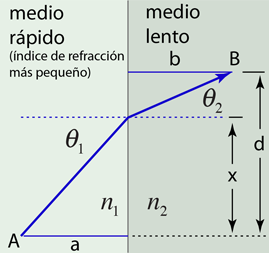
\includegraphics[width=4cm]{imagenes/fer5.png}
    \caption{\textbf{Diagrama de refracción.} En el se observan dos medios con índices de refracción distintos y un rayo incidente que al pasar por el segundo medio el ángulo del rayo cambia \cite{pagina}}
    \label{fig:my_label}
\end{figure}
Todo lo anterior se escribe como \cite{book} 
\begin{equation*}
    n_T \sin{\theta_T} =  n_I \sin{\theta_I} 
\end{equation*}

o bien

\begin{equation}
    \sin{\theta_T} =  \frac{n_I}{n_T} \sin{\theta_I} 
\end{equation}

\begin{equation}
    \sin{\theta_T} = \frac{v_T}{v_I} \sin{\theta_I}
\end{equation}

Esto porque:
\begin{equation}
    \frac{n_I}{n_T} = \frac{v_T}{v_I}
\end{equation}


\section*{\textcolor{carmine}{Desarrollo Experimental}}
\subsection*{\textcolor{carmine}{Aire-Lucita}}
Sobre la mesa del laboratorio se colocó un goniómetro con un láser. Se encendió el láser y fue alineado con el centro del circulo, se detectó que la incertidumbre para los ángulos estaría dada por la mitad de la mínima escala es decir $\sigma_{ap}=\pm 0.5^{\circ}$. Con mucho cuidado se situó la lucita sobre el semicírculo del goniómetro de tal manera en que el medio del rayo incidente fuera el aire como se muestra en la figura 3(a).
\\
Para comprobar la ley de reflexión se tomaron los ángulos del rayo incidente y del rayo reflejado con la normal,  partiendo de $5^{\circ}$ y variando de $5^{\circ}$ en $5^{\circ}$ como se muestra en la figura 3(b).
\\
Para la ley de la refracción se tomaron los ángulos del rayo incidente y del rayo refractado con su respectiva normal, partiendo de $5^{\circ}$ y variando de $5^{\circ}$ en $5^{\circ}$.

\begin{figure}[H]
 \centering
  \subfloat[\textbf{Montaje del dispositivo experimental.} La lucita se colocó frente al láser para que el medio del rayo incidente fuera el aire, con el goniómetro se midieron los ángulos de interés.]{
   \label{f:Lambert1}
    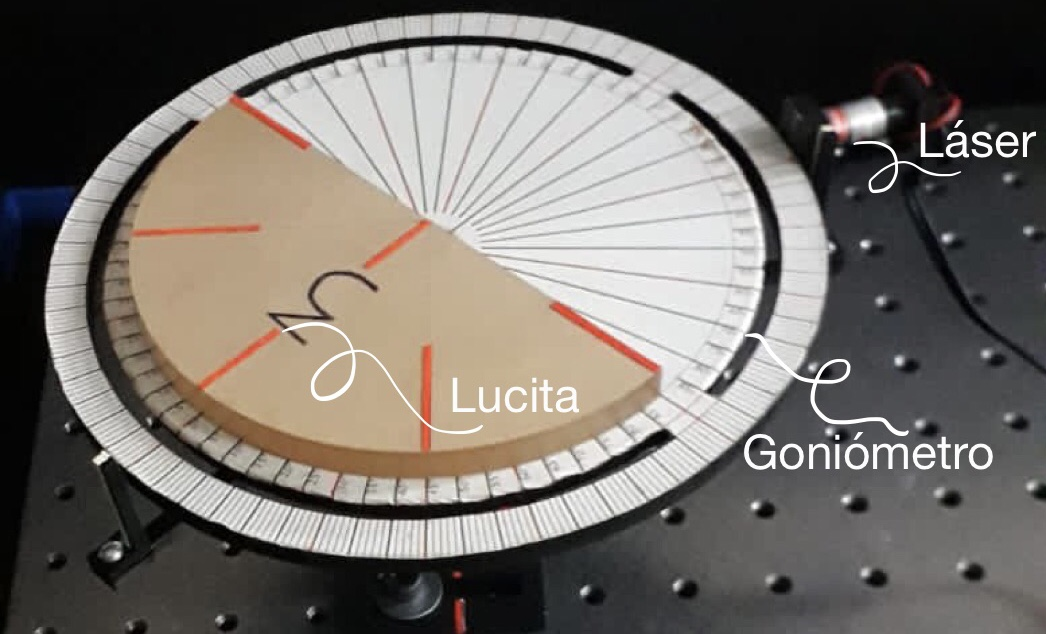
\includegraphics[width=0.36\textwidth]{imagenes/6A655C8B-B727-4DC7-A004-815A41EF1525.jpeg}}
  \subfloat[\textbf{Funcionamiento del dispositivo experimental.} Se muestra el láser que se refleja y se refracta usando al aire como medio incidente.]{
   \label{f:Lambert2}
    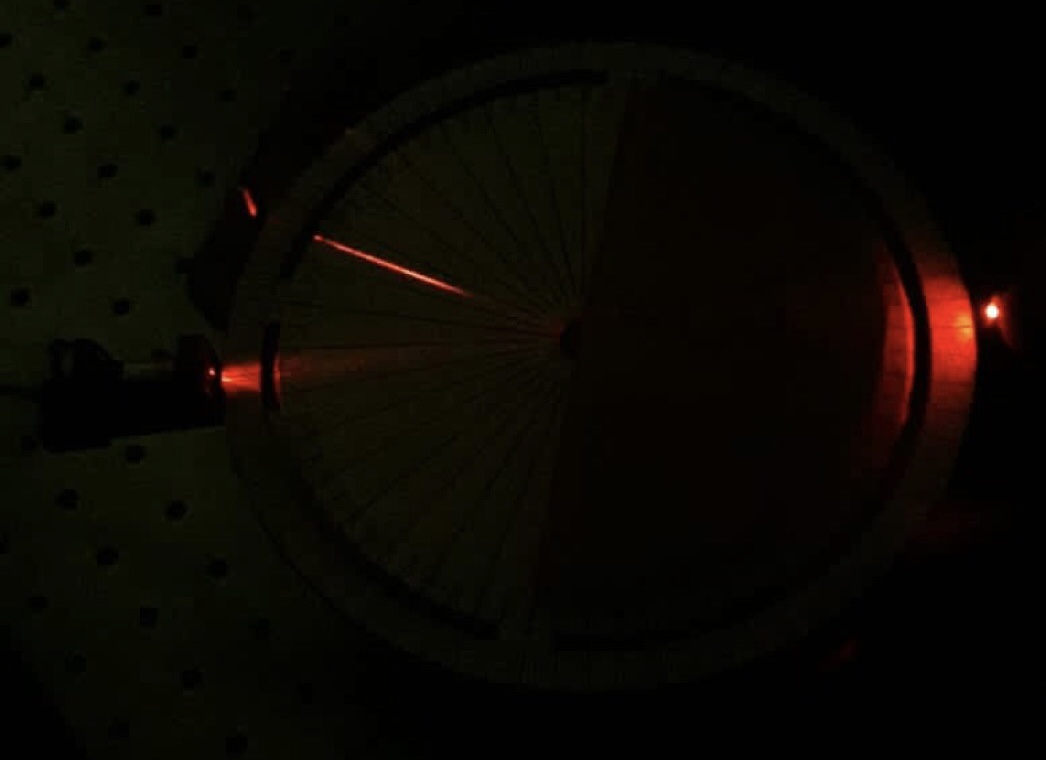
\includegraphics[width=0.3\textwidth]{imagenes/7AB76497-7C3B-4FE7-9818-60ED9F04D0E3.jpeg}}
    \caption{Dispositivo experimental con el aire como medio del rayo incidente.}
     \label{f:Lambert3}
\end{figure}
\subsection*{\textcolor{carmine}{Lucita-Aire}}
Con el arreglo experimental anterior, se cambió la lucita como medio del rayo incidente, como se muestra en la figura 4. Se cuidó que el láser estuviera  alineado como en el experimento anterior.\\
Para comprobar la ley de reflexión se tomaron los ángulos del rayo incidente y del rayo reflejado con la normal,  partiendo de $5^{\circ}$ y variando de $5^{\circ}$ en $5^{\circ}$.
\\
Para la ley de la refracción se tomaron los ángulos del rayo incidente y del rayo refractado con su respectiva normal, partiendo de $5^{\circ}$ y variando de $5^{\circ}$ en $5^{\circ}$. En este caso se encontró que en $47^{\circ}\pm1^{\circ}$ desaparecía el rayo refractado por lo que se le nombró el ángulo critico.
\begin{figure}[H]
    \centering
    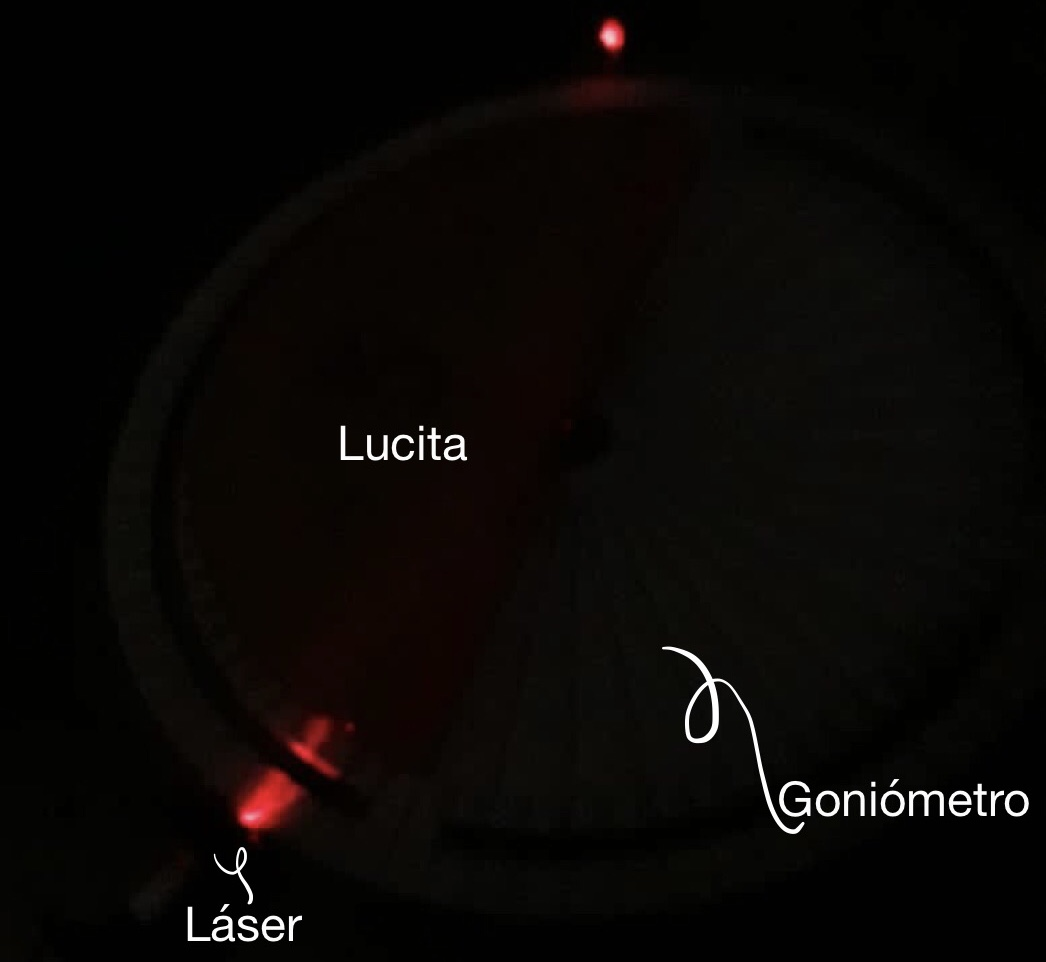
\includegraphics[width=6cm]{imagenes/B83169D6-410E-4924-B0E5-842D628921D4.jpeg}
    \caption{\textbf{Montaje experimental para el caso Lucita-Aire.} La lucita se colocó frente al láser y se midieron los ángulos con  el goniómetro.}
    \label{fig:my_label}
\end{figure}




\section*{\textcolor{carmine}{Resultados y Análisis.}}


\begin{figure}[h!]
 \centering
  \subfloat[Gráfica del ángulo de reflexión $\theta_T$ vs el ángulo de incidencia $\theta_I$ con el aire como medio incidente y lucita como medio reflector.]{
   \label{f:Lambert1}
    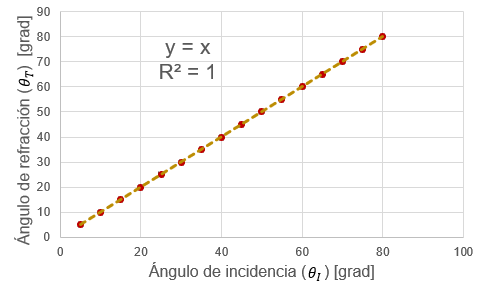
\includegraphics[width=0.4\textwidth]{graficas/aire_lucita_reflexion.PNG}}
  \subfloat[Gráfica del ángulo de reflexión $\theta_T$ vs el ángulo de incidencia $\theta_I$ con la lucita como medio incidente y aire como medio reflector.]{
   \label{f:Lambert2}
    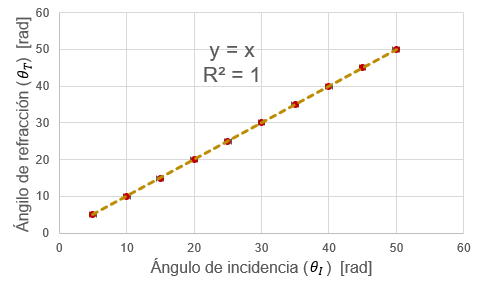
\includegraphics[width=0.4\textwidth]{graficas/lucita_aire_reflexion.PNG}}
    \caption{Gráficas de reflexión para aire-lucita y lucita-aire.}
     \label{f:Lambert3}
\end{figure}

De los datos que se obtuvieron para comprobar la ley de la reflexión se puede observar que los ángulos cumplen con una relación de la forma:

\begin{equation*}
   \theta_{T}=m\theta_{I}
\end{equation*}

\begin{equation*}
  \iff m= \frac{\theta_{T}}{\theta_{I}}
\end{equation*}

Mediante el método de mínimos cuadrados se tiene que:
\begin{equation*}
    m = 1.00
\end{equation*}

La pendiente obtenida no presenta incertidumbre estadística, solo tiene una incertidumbre nominal dada por:
\begin{equation*}
   \delta m=\sqrt{\left( \frac{\partial m}{\partial \theta_{T}} \delta \theta_{T}\right)^2 +\left( \frac{\partial m}{\partial \theta_{I}} \delta \theta_{I}\right)^2 }
\end{equation*}

\begin{equation*}
    =\sqrt{\left( \frac{1}{\theta_{I}} \delta \theta_{T}\right)^2 +\left( -\frac{\theta_{T}}{\theta_{I}^2} \delta \theta_{I}\right)^2 }
\end{equation*}
Sustituyendo a $\theta_{T}=\theta_{I}=5^{\circ}$ con $\delta \theta_{T}=\delta \theta_{I}=0.5^{\circ} $ y simplificando se tiene:

\begin{equation*}
   \delta m = \pm 0.14
\end{equation*}

De esta manera:

\begin{equation*}
   \theta_{T}=(1.00\pm0.14)\theta_{I}
\end{equation*}

\begin{figure}[H]
 \centering
  \subfloat[Gráfica del seno del ángulo de refracción $\theta_T$ vs el seno del ángulo de incidencia $\theta_I$ con aire como medio incidente y lucita como medio refractor.]{
   \label{f:Lambert1}
    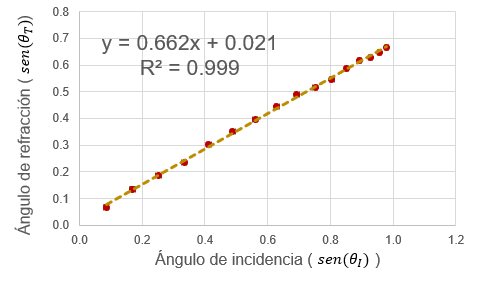
\includegraphics[width=0.4\textwidth]{graficas/aire_lucita_refraccion.PNG}}
  \subfloat[Gráfica del seno del ángulo de refracción $\theta_T$ vs el seno del ángulo de incidencia $\theta_I$ con lucita como medio incidente y aire como medio refractor.]{
   \label{f:Lambert2}
    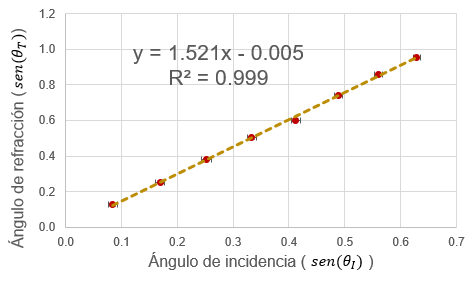
\includegraphics[width=0.4\textwidth]{graficas/lucita_aire_refraccion.PNG}}
    \caption{Gráficas de ecuación linealizada (3) para refracción aire-lucita y lucita-aire.}
     \label{f:Lambert3}
\end{figure}

Utilizando el método de mínimos cuadrados en los datos del experimento de la refracción se obtuvo que:

\begin{equation*}
    m_{1}=(0.662 \pm 0.005)
\end{equation*}

\begin{equation*}
    m_{2} = (1.521 \pm 0.018)
\end{equation*}

Con estas pendientes se obtienen las respectivas ecuaciones:

\begin{equation*}
    \sin{\theta_{Taire}}=(0.662 \pm 0.005)\sin{\theta_{Ilucita}}
\end{equation*}

\begin{equation*}
    \sin{\theta_{Tlucita}}=(1.521 \pm 0.018)\sin{\theta_{Iaire}}
\end{equation*}
%Ya estan bien las ecuaciones.
De la teoría se tiene que se debe de cumplir:
$$ \frac{n_{lucita}}{n_{aire}}= (1.521 \pm 0.018)$$
$$ \frac{n_{aire}}{n_{lucita}}= (0.662 \pm 0.005)$$
Comparando con los valores exactos: % propuestos en la literatura \cite{hipotesis}:
$$ \frac{n_{lucita}}{n_{aire}}= 1.5 $$
$$ \frac{n_{aire}}{n_{lucita}}= 0.667 $$
Se puede ver que la ley de refracción se cumple, donde $n_{aire}=1$, $n_{lucita}=1.5$.
\\
Ahora, de la teoría se sabe  que:
\begin{equation*}
    v_{lucita}= m_{1} \cdot v_{aire}
\end{equation*}
Y con:
\begin{equation*}
    v_{lucita2}= v_{aire} / m_{2}
\end{equation*}

Utilizando $v_{aire} = 299705543 \frac{m}{s}$ en la primera formula, $v_{lucita}$, se encontró:

%con $v_I=c= 3\times 10^{8}$

\begin{equation*}
    v_{lucita}  = 1.986 \times 10^{8} \frac{m}{s} 
\end{equation*}

Donde la incertidumbre esta dada por la formula de propagación de errores:

\begin{equation*}
    \delta v_{lucita} = \sqrt{\left(\frac{\partial v_{lucita}}{\partial m}\right)^2\delta m^2}
\end{equation*}

\begin{equation*}
    = v_{aire} \cdot \delta m
\end{equation*}

Sustituyendo los valores y simplificando:

\begin{equation*}
\delta v_{lucita} = 1.5 \times 10^{6} \frac{m}{s}
\end{equation*}

Ahora utilizando $v_{aire} = 299705543 \frac{m}{s}$ en la segunda formula, $v_{lucita2}$, se encontró:

%con $v_T = c = 3\times 10^{8}$

\begin{equation*}
    v_{lucita2} = 1.972 \times 10^{8} \frac{m}{s}
\end{equation*}
Con incertidumbre:

\begin{equation*}
    \delta v_{lucita2} = \sqrt{\left(\frac{\partial v_{lucita2}}{\partial m_{2}}\right)^2\delta m^2} 
\end{equation*}

\begin{equation*}
    = \frac{v_{aire}}{m_{2}^2} \delta m
\end{equation*}
Sustituyendo los valores y simplificando:
\begin{equation*}
    \delta v_{lucita2}= 2.3 \times 10^{6} \frac{m}{s}
\end{equation*}

Promediando ambos resultados y sumando por cuadraturas las incertidumbres se obtiene una velocidad de la luz en la lucita de:

\begin{equation*}
    v= (1.979 \pm 0.028) \times 10^{8} \frac{m}{s}
\end{equation*}


\section*{\textcolor{carmine}{Discusión y Conclusión.}}
\nocite{*}
Se obtuvo:
\begin{equation*}
   \theta_{T}=(1.00\pm0.14)\theta_{I}
\end{equation*}
%Se concluye que la ley de reflexión (ecuación 1) se cumple debido a que las pendientes presentes en la figura 5 cumplen con la misma.
Con esto se puede concluir que la ley de reflexión se cumple para este caso especifico.
\\
Tambien se obtuvo que:
$$ \frac{n_{lucita}}{n_{aire}}= (1.521 \pm 0.018)$$
$$ \frac{n_{aire}}{n_{lucita}}= (0.662 \pm 0.005)$$
Comparando con los valores exactos: % propuestos en la literatura \cite{hipotesis}:
$$ \frac{n_{lucita}}{n_{aire}}= 1.5 $$
$$ \frac{n_{aire}}{n_{lucita}}= 0.667 $$
Se puede ver que la ley de refracción se cumple para los medios especificos aire-lucita y lucita-aire.
\\
Se obtuvo que la velocidad de la luz en la lucita es:

\begin{equation*}
    v= (1.979 \pm 0.028) \times 10^{8} \frac{m}{s}
\end{equation*}

El error entre la velocidad obtenida y el valor propuesto en la literatura  es de $1.28$ ($<2$) veces la incertidumbre absoluta por lo que es un resultado satisfactorio y además verifica que se cumple la ley de refracción propuesta en la introducción. % este criterio es necesario si quieren lo pueden reescribir pero no lo quiten por favor. 

El valor que se obtuvo  para la velocidad de la lucita es tan solo una aproximación al valor real, los instrumentos que se utilizan en el laboratorio no cuentan con escalas suficientes para dar un valor preciso ni exacto, el fin de estas practicas es aprender los métodos básicos con los que se hacen mediciones.


\bibliography{biblio}
\newpage
\section*{\textcolor{carmine}{Apéndice}}

\begin{multicols}{2}

\begin{Figura}
    \centering
    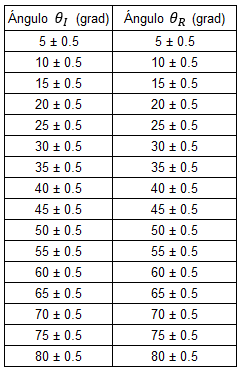
\includegraphics[width=0.5 \textwidth]{tablas/tabla aire_lucita_reflexion.PNG}
    \captionof{table}{Ángulos de incidencia y reflexión obtenidos  en el caso aire-lucita}
    \label{fig}
\end{Figura}

\begin{Figura}
    \centering
    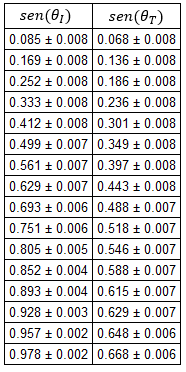
\includegraphics[width=0.4 \textwidth]{tablas/tabla aire_lucita_refraccion.PNG}
    \captionof{table}{Datos obtenidos aplicando la función $\sin{\theta}$ a los ángulos de incidencia y refracción registrados para el caso aire-lucita}
    \label{fig}
\end{Figura}
%%
\begin{Figura}
    \centering
    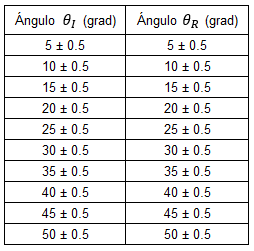
\includegraphics[width=0.5 \textwidth]{tablas/tabla lucita_aire_reflexion.PNG}
    \captionof{table}{Ángulos de incidencia y reflexión obtenidos  en el caso aire-lucita}
    \label{fig}
\end{Figura}

\begin{Figura}
    \centering
    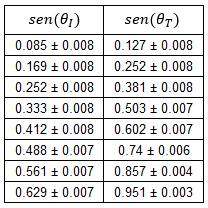
\includegraphics[width=0.5 \textwidth]{tablas/tabla lucita_aire_refraccion.PNG}
    \captionof{table}{Datos obtenidos aplicando la función $\sin{\theta}$ a los ángulos de incidencia y refracción registrados para el caso lucita-aire}
    \label{fig}
\end{Figura}


\end{multicols}
\end{document}
